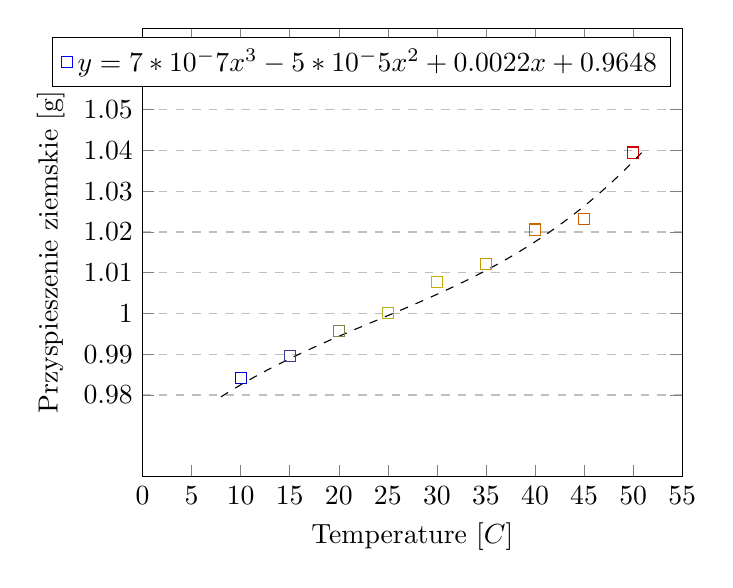
\begin{tikzpicture}
	\begin{axis}[
			xlabel={Temperature [$\degree C$]},
			ylabel={Przyspieszenie ziemskie [g]},
			xmin=0, xmax=55,
			ymin=0.96, ymax=1.07,
			xtick={0,5,10,15,20,25,30,35,40,45,50,55},
			ytick={0.98,0.99,1,1.01,1.02,1.03,1.04,1.05},
			ymajorgrids=true,
			grid style=dashed,
		]
																																																																																																		
		\addplot+[
			only marks,
			scatter,
			color=blue,
			mark=square,
		]
		coordinates {
			(10,0.9842)(15,0.9895)(20,0.9957)(25,1.0002)(30,1.0077)(35,1.0122)(40, 1.0206)(45, 1.0232)(50, 1.0395)
		};
											
		\addplot [
			dashed,
			domain=8:51, 
			samples=90, 
			color=black,
		]
		{0.0000007*x^3 - 0.00005*x^2 + 0.0022*x + 0.9648};
		\legend{$y = 7*10^-7 x^3 - 5*10^-5 x^2 + 0.0022x + 0.9648$}
	\end{axis}
\end{tikzpicture}	